\documentclass[11pt,ngerman,a4paper]{article}
%Gummi|061|=)
\usepackage{amsmath}
\usepackage{a4wide}
\usepackage{url}
\usepackage{amsthm}
\usepackage{amsbsy}
\usepackage{amssymb}
\usepackage{inputenc}
\usepackage{rotating} 
\usepackage{here}
\usepackage{graphicx}
\usepackage{paralist}
\usepackage{selinput}
\usepackage[separate-uncertainty=true]{siunitx}
\usepackage{booktabs}
\sisetup{}
\SelectInputMappings{%
adieresis={ä},
germandbls={ß},
}
\title{\textbf{Versuch V308: Spulen und Magnetfelder}}
\author{Martin Bieker\\
		Julian Surmann\\
		\\
		Durchgef\"{u}hrt am 20.05.2014\\
		TU Dortmund}
\date{}
\usepackage{graphicx}
\begin{document}
\renewcommand\tablename{Tabelle}
\renewcommand\figurename{Abbildung}
\maketitle
\thispagestyle{empty}
\newpage
\clearpage
\setcounter{page}{1}


\section{Einleitung}
In diesem Versuch soll der Verlauf der magnetischen Feldstärke in verschiedenen Spulenanordnungen gemessen werden. 
\section{Theorie}
Magnetfelder entstehen durch die Bewegung elektrischer Ladungen. Also wird jeder Leiter, durch den ein elektrischer Strom fließt, von einem Magnetfeld umgeben. Im Gegensatz zu E-Feld-Linien sind Magnetfeldlinien immer geschlossen. Außerdem kreuzen sie sich nicht. Im Falle einer in diesem Versuch betrachteten Spule beschreiben die Feldlinien konzentrische Kreise, die senkrecht zum Stromfluss verlaufen.

\subsection{Magnetfeld einer langen Spule}
Das Magnetfeld im Innern eine langen Spule kann als homogen angesehen werden. Nimmt man den Raum ausserhalb der Spule als feldfrei an, so kann die Stärke das magnetischen Feldes näherungsweise mit Hilfe der \textsc{4. Maxwellgleichung} 
\begin{equation}
\oint B\cdot d\vec r = \mu_r\mu_0 I
\end{equation}
berechnet werden. Es ergibt sich:
\
\begin{equation}
B = \mu_r\mu_0\frac{nI}l\mathrm.
\end{equation}
\subsection{Magnetfeld einer Helmholtz-Spule}
Bei einer Helmholtz-Spule haben zwei Spulen als Abstand zueinander ihren Radius. Bei dieser Anordnung wird auf der Spulenachse im Inneren ein homogenes Magnetfeld erzeugt. Dieses Magnetfeld hat die selben Eigenschaften wie das Magnetfeld einer langen Spule, allerdings ist es für Versuche oft besser geeignet, da zwischen dem Helmholtz-Spulenpaar ein Versuchsaufbau arretiert werden kann. Ein Helmholtz-Spulenpaar ist in Abbildung \ref{hhspule} dargestellt.


\begin{figure}[htp]
\centering
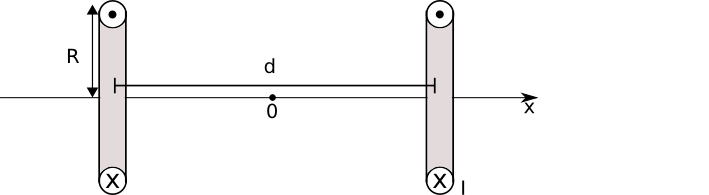
\includegraphics[scale=1.00]{helmholtz.png}
\caption{Schematische Darstellung eines Helmholtz-Spulenpaars}
\label{hhspule}
\end{figure}
\noindent
Die Magnetfeldstärke auf der Spulenachse an der Stelle x wird dann berechnet mit 
\begin{equation}
\vec B(x)= \frac{\mu_0I}{2}\left(\frac1{\left(R^2 + (x+\frac d2)^2 \right)^\frac32} + \frac1{\left(R^2 + (x-\frac d2)^2 \right)^\frac32}  \right) \cdot \vec e_x.
\label{BFeld}
\end{equation}
Wenn man Formel (\ref{BFeld}) nach x ableitet, ergibt sich die Änderung der Magnetfeldstärke B:
\begin{equation}
\frac{d\vec B}{d x} = \frac{-3\mu_0I}{2}\left( \frac{x+\frac d2}{\left(R^2 + (x+\frac d2)^2 \right)^\frac52} + \frac{x-\frac d2}{\left(R^2 + (x-\frac d2)^2 \right)^\frac52}\right) \cdot \vec e_x.
\end{equation}
\subsection{Funktionsweise einer Hall-Sonde}
Die in diesem Versuch zu bestimmenden magnetischen Feldstärken, werden mit Hilfe einer Hall-Sonde gemessen. Dieses Messverfahren basiert auf dem \textit{Hall-Effekt}, welcher an dieser Stelle kurz durch Abbildung \ref{hall} erläutert werden soll.  

\begin{figure}[htp]
\centering
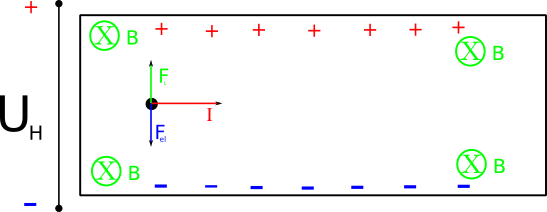
\includegraphics[scale=1.00]{hall.png}
\caption{Schematische Darstellung des Hall-Effekts}
\label{hall}
\end{figure}
\noindent
An die Hallsonde wird ein Strom $I$ angelegt. Wird die Sonde von einem magnetischen Feld $\vec B$ durchdrungen, werden die bewegten Ladungen im Inneren durch die Lorentzkraft $F_L$ abgelenkt. Auf Grund dieser Ladungstrennung entsteht ein Elektisches Feld $\vec E$. Dieses wirkt der Ansammlung weiterer Ladungsträger entgegen. Des Weiteren wird durch das Feld eine Spannung erzeugt, die an den Seiten der Sonde abgegriffen werden kann. Im Gleichgewicht gilt:
\[
F_L = F_{el}.
\]
Hieraus kann eine Beziehung für das Magnetfeld in Abhängigkeit von der gemessenen Spannung $U_H$ hergeleitet werden:
\[
B = \frac{d}{A_H I } \cdot U_H.
\]
Dabei ist $A_H$, genannt Hallkonstante, eine Materialkonstante und $d$ die Dicke der Hall-Sonde. 
Diese Berechnungen werden vom Messgerät, welches in diesem Versuch verwendet wird, intern ausgeführt. Die so gemessene magnetische Feldstärke wird also direkt angezeigt.

\section{Aufbau und Durchführung}
Alle Spulen werden an Labornetzteilen angeschlossen, die die Spannung und den fließenden Strom zeigen. Zur Messung der Magnetfeldstärke wird eine Hallsonde an ein Gaußmeter angeschlossen.
\subsection{Messung an der langen Spule}
Für die Messung an der langen Spule stehen drei Spulenmodule zur Verfügung. Die Spulen sind identisch zueinander und haben folgende Eigenschaften:
\begin{itemize}
\item $n = 3400$
\item $d = \SI{0.11}{\meter} \Rightarrow r =  \SI{0.055}{\meter} $.
\end{itemize}
Die Module können hintereinander gesetzt werden, um so längere Spulen zu erzeugen. Die zu vermessende Spule kann an einem Holzlineal auf der x-Achse verschoben werden. Eine longitudinale Hallsonde ist so an einem Stativ befestigt, dass die Sonde auf der Achse der Spule liegt. Durch das Verschieben der Spule wird dann das Magnetfeld im Inneren der Spule an verschiedenen Punkten der Achse gemessen.
\newline
Es werden drei Spulen mit unterschiedlicher Länge untersucht. Dabei wird die Magnetfeldstärke in Abhängigkeit vom Ort x der Hallsonde gemessen.
\subsection{Messung an der Helmholtz-Spule}
Das Spulenpaar ist auf einem Sockel befestigt, der an einer Skala das Ablesen der Spulenpositionenen ermöglicht. Über den Spulen befindet sich eine Schiene zur Aufnahme der transversalen Hallsonde. An dieser Schiene befindet sich ebenfalls eine Skala. Die Spulen haben folgende Eigenschaften:
\begin{itemize}
\item $n = 100$
\item $l = \SI{0.033}{\meter}$
\item $d = \SI{0.125}{\meter} \Rightarrow r =  \SI{0.0625}{\meter} $.
\end{itemize}
Es werden nun drei verschiedene Spulenabstände untersucht, bei einem dieser Abstände soll der Abstand der Spulen gleich dem Radius der Spulen sein. Dann handelt es sich um ein Helmholtz-Spulenpaar und das Magnetfeld auf der Spulenachse soll homogen sein. Es sollen jeweils 15 Magnetfeldstärken an verschiedenen Orten x auf der Spulenachse gemessen werden.

\section{Auswertung}
Die in den Tabellen 1-6 (Anhang) sind die gemessenen Werte eingetragen. Mit Hilfe der Formel (3) wurden dann die Theoriekurven des Spulenpaars und mit Hilfe der Formel (2) die Theoriekurven der langen Spule berechnet. Dabei wurden folgende Größen eingesetzt:
\begin{itemize}
\item $n_{Spulenpaar} = 100$
\item $R_{Spulenpaar} = \SI{0.125}{\meter}$
\item $I_{Spulenpaar} = \SI{2.78}{\ampere}$
\item $n_{Spulenelement} = 3400$
\item $R_{Spulenelement} = \SI{0.055}{\meter}$
\item $I_{lange Spule} = \SI{0.7}{\ampere}$
\item $I_{mittlere, kurze Spule} = \SI{0.8}{\ampere}$
\item $l_{Spulenelement} \approx \SI{0.1}{\meter}$
\end{itemize}
Die gemessenen und berechneten Kurven sind jeweils in den Abbildungen \ref{plot1} bis \ref{plot6} abgebildet. Dabei sind die Graphen so verschoben, dass bei $x=0$ der Mittelpunkt der Spule/Spulen ist.


\begin{figure}[htp]
\centering
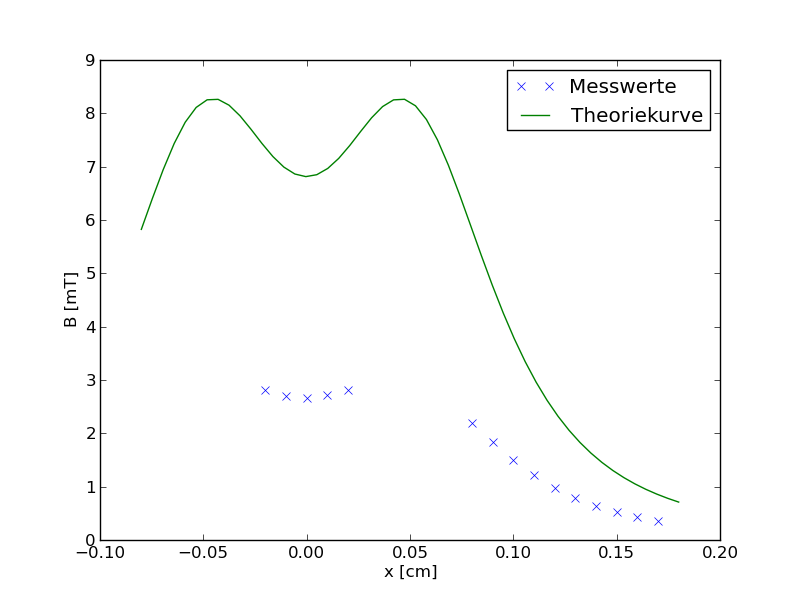
\includegraphics[scale=0.7]{e11.png}
\caption{Spulenpaar - $d =\SI{0.1}{\meter}$}
\label{plot1}
\end{figure}

\begin{figure}[htp]
\centering
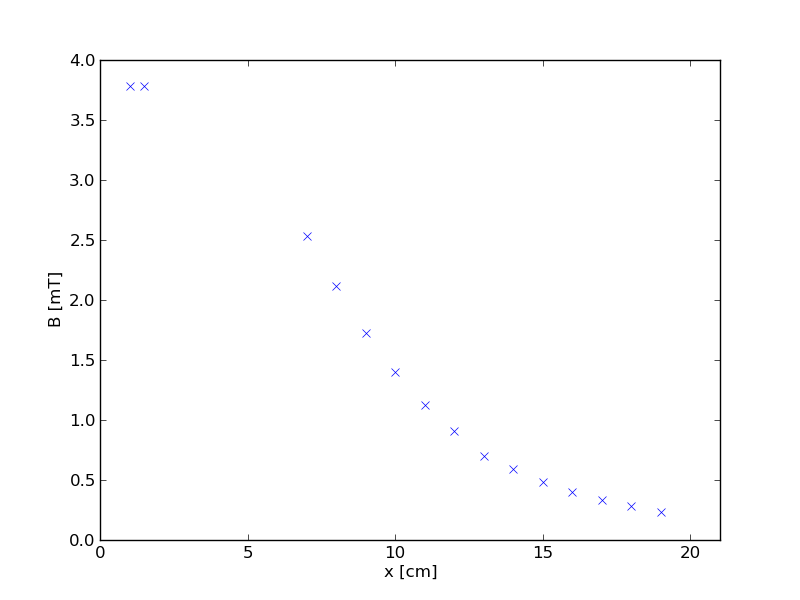
\includegraphics[scale=0.7]{e12.png}
\caption{Spulenpaar - $d =\SI{0.0625}{\meter}$}
\label{hhspule}
\end{figure}

\begin{figure}[htp]
\centering
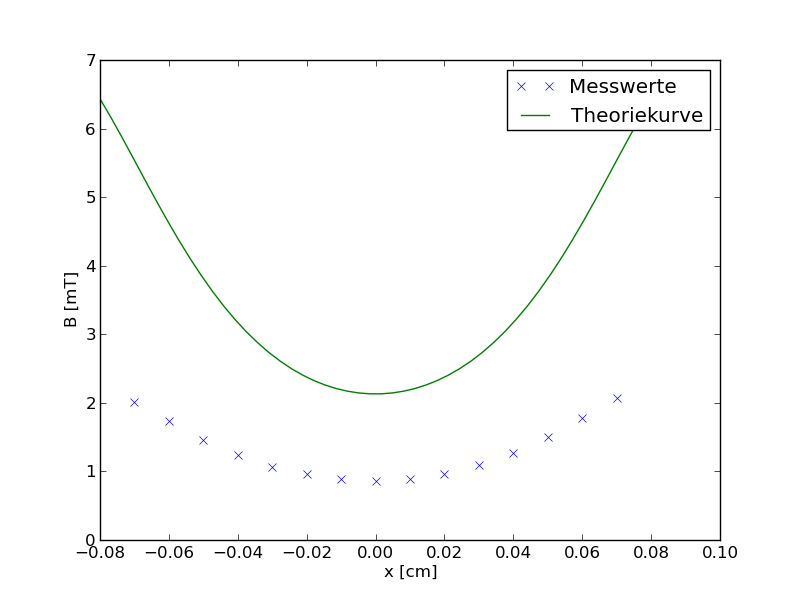
\includegraphics[scale=0.7]{e13.png}
\caption{Spulenpaar - $d =\SI{0.2}{\meter}$}
\label{hhspule}
\end{figure}

\begin{figure}[htp]
\centering
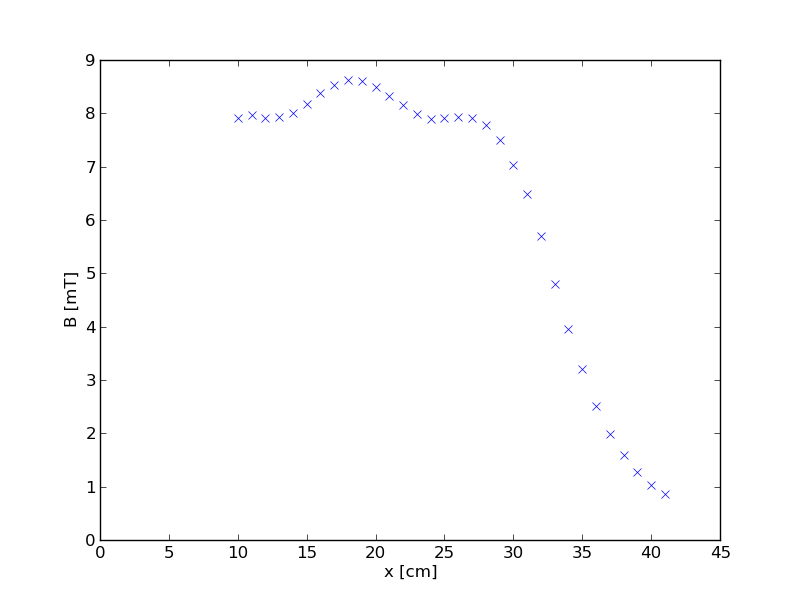
\includegraphics[scale=0.7]{e21.png}
\caption{Lange Spule (drei Elemente)}
\label{hhspule}
\end{figure}

\begin{figure}[htp]
\centering
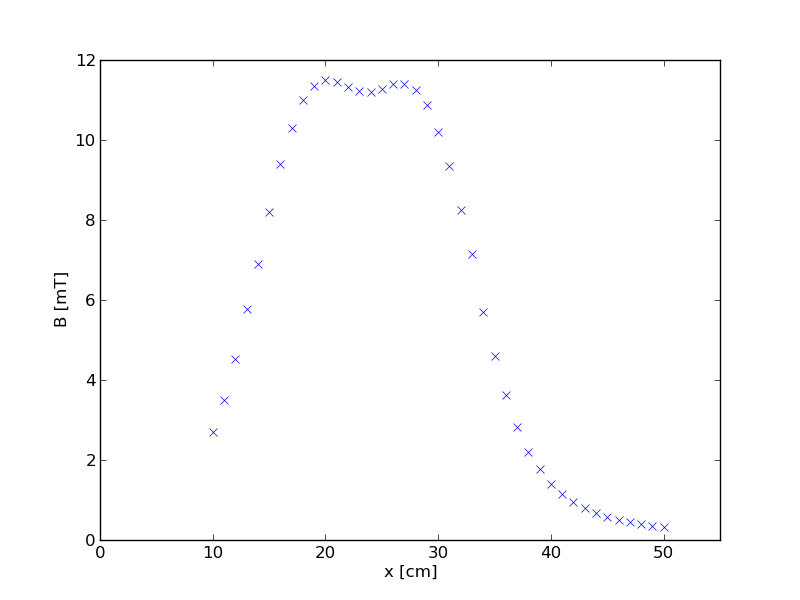
\includegraphics[scale=0.7]{e22.png}
\caption{Mittlere Spule (zwei Elemente)}
\label{hhspule}
\end{figure}

\begin{figure}[htp]
\centering
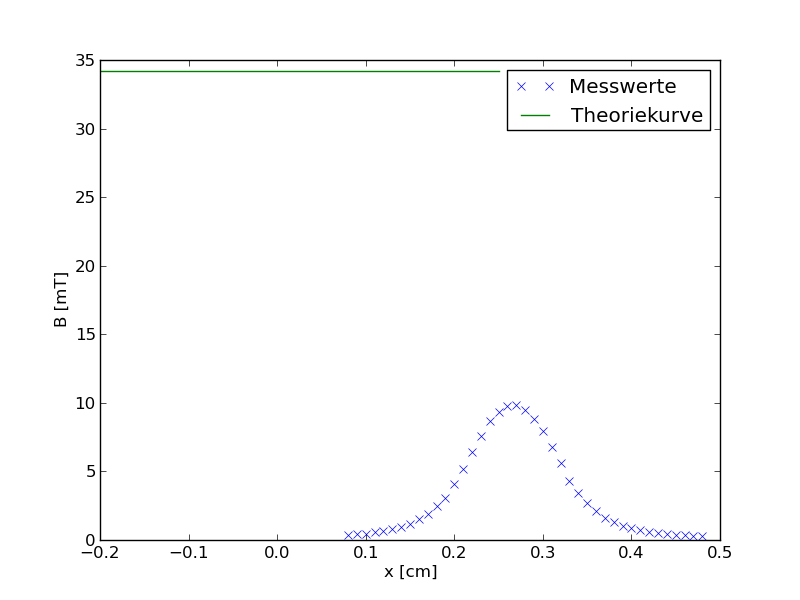
\includegraphics[scale=0.7]{e23.png}
\caption{Kurze Spule (ein Element)}
\label{plot6}
\end{figure}

\section{Diskussion}
Die Messung der Magnetfeldstärke mit Hilfe der Hallsonde war gut durchzuführen. Die Werte wurden in mT digital ausgegeben.
\newline


\section{Quellen}
\begin{enumerate}[{[}1{]}]
\item Entnommen der Praktikumsanleitung \textit{V308: Spulen und Magnetfelder} der TU Dortmund. Download am 26.05.14 unter:\\
 \url{http://129.217.224.2/HOMEPAGE/PHYSIKER/BACHELOR/AP/SKRIPT/Magnetfeld.pdf}
\end{enumerate}

\section{Anhang}
\begin{itemize}
\item Tabellen
\item Auszug aus dem Messheft
\end{itemize}
\newpage

\begin{table}[H]
\centering
\begin{tabular}{ll}
\toprule
{$x / \si{\centi\meter}$} &{ $B/\si{\milli\tesla}$ }\\
\midrule
1.0 & 2.805\\
2.0 & 2.705\\
3.0 & 2.668\\
4.0 & 2.712\\
5.0 & 2.819\\
11.0 & 2.195\\
12.0 & 1.844\\
13.0 & 1.507\\
14.0 & 1.215\\
15.0 & 0.972\\
16.0 & 0.779\\
17.0 & 0.633\\
18.0 & 0.517\\
19.0 & 0.422\\
20.0 & 0.347\\
\bottomrule
\end{tabular}
\label{}
\caption{Untersuchung des Spulenpaares - $d =\SI{0.1}{\meter}$}
\end{table}

\begin{table}[H]
\centering
\begin{tabular}{ll}
\toprule
{$x / \si{\centi\meter}$} &{ $B/\si{\milli\tesla}$ }\\
\midrule
1.0 & 3.782\\
1.5 & 3.78\\
7.0 & 2.531\\
8.0 & 2.118\\
9.0 & 1.727\\
10.0 & 1.403\\
11.0 & 1.123\\
12.0 & 0.907\\
13.0 & 0.701\\
14.0 & 0.594\\
15.0 & 0.485\\
16.0 & 0.402\\
17.0 & 0.336\\
18.0 & 0.282\\
19.0 & 0.237\\
\bottomrule
\end{tabular}
\label{}
\caption{Untersuchung des Spulenpaares - $d =\SI{0.0625}{\meter}$}
\end{table}

\begin{table}[H]
\centering
\begin{tabular}{ll}
\toprule
{$x / \si{\centi\meter}$} &{ $B/\si{\milli\tesla}$ }\\
\midrule
1.0 & 2.01\\
2.0 & 1.729\\
3.0 & 1.464\\
4.0 & 1.244\\
5.0 & 1.067\\
6.0 & 0.957\\
7.0 & 0.886\\
8.0 & 0.867\\
9.0 & 0.892\\
10.0 & 0.967\\
11.0 & 1.09\\
12.0 & 1.268\\
13.0 & 1.499\\
14.0 & 1.785\\
15.0 & 2.073\\
\bottomrule
\end{tabular}
\label{}
\caption{Untersuchung des Spulenpaares - $d =\SI{0.2}{\meter}$}
\end{table}

\begin{table}[H]
\centering
\begin{tabular}{ll}
\toprule
{$x / \si{\centi\meter}$} &{ $B/\si{\milli\tesla}$ }\\
\midrule
10.0 & 7.92\\
11.0 & 7.96\\
12.0 & 7.92\\
13.0 & 7.93\\
14.0 & 8.01\\
15.0 & 8.17\\
16.0 & 8.39\\
17.0 & 8.54\\
18.0 & 8.63\\
19.0 & 8.61\\
20.0 & 8.5\\
21.0 & 8.33\\
22.0 & 8.15\\
23.0 & 7.99\\
24.0 & 7.9\\
25.0 & 7.91\\
26.0 & 7.94\\
27.0 & 7.92\\
28.0 & 7.79\\
29.0 & 7.5\\
30.0 & 7.03\\
31.0 & 6.49\\
32.0 & 5.7\\
33.0 & 4.8\\
34.0 & 3.96\\
35.0 & 3.2\\
36.0 & 2.51\\
37.0 & 1.98\\
38.0 & 1.59\\
39.0 & 1.27\\
40.0 & 1.04\\
41.0 & 0.86\\
\bottomrule
\end{tabular}
\label{}
\caption{Untersuchung der langen Spule (drei Elemente)}
\end{table}

\begin{table}[H]
\centering
\begin{tabular}{ll}
\toprule
{$x / \si{\centi\meter}$} &{ $B/\si{\milli\tesla}$ }\\
\midrule
10.0 & 2.71\\
11.0 & 3.49\\
12.0 & 4.53\\
13.0 & 5.78\\
14.0 & 6.89\\
15.0 & 8.2\\
16.0 & 9.4\\
17.0 & 10.31\\
18.0 & 11.0\\
19.0 & 11.36\\
20.0 & 11.5\\
21.0 & 11.46\\
22.0 & 11.33\\
23.0 & 11.22\\
24.0 & 11.2\\
25.0 & 11.28\\
26.0 & 11.39\\
27.0 & 11.41\\
28.0 & 11.26\\
29.0 & 10.88\\
30.0 & 10.19\\
31.0 & 9.34\\
32.0 & 8.24\\
33.0 & 7.14\\
34.0 & 5.7\\
35.0 & 4.6\\
36.0 & 3.63\\
37.0 & 2.83\\
38.0 & 2.2\\
39.0 & 1.77\\
40.0 & 1.41\\
41.0 & 1.14\\
42.0 & 0.96\\
43.0 & 0.81\\
44.0 & 0.68\\
45.0 & 0.58\\
46.0 & 0.51\\
47.0 & 0.45\\
48.0 & 0.4\\
49.0 & 0.35\\
50.0 & 0.32\\
\bottomrule
\end{tabular}
\label{}
\caption{Untersuchung der mittleren Spule (zwei Elemente)}
\end{table}

\begin{table}[H]
\centering
\begin{tabular}{ll}
\toprule
{$x / \si{\centi\meter}$} &{ $B/\si{\milli\tesla}$ }\\
\midrule
10.0 & 0.35\\
11.0 & 0.42\\
12.0 & 0.47\\
13.0 & 0.55\\
14.0 & 0.66\\
15.0 & 0.81\\
16.0 & 0.97\\
17.0 & 1.19\\
18.0 & 1.5\\
19.0 & 1.9\\
20.0 & 2.45\\
21.0 & 3.09\\
22.0 & 4.09\\
23.0 & 5.15\\
24.0 & 6.45\\
25.0 & 7.61\\
26.0 & 8.66\\
27.0 & 9.35\\
28.0 & 9.8\\
29.0 & 9.86\\
30.0 & 9.49\\
31.0 & 8.83\\
32.0 & 7.93\\
33.0 & 6.79\\
34.0 & 5.58\\
35.0 & 4.31\\
36.0 & 3.43\\
37.0 & 2.71\\
38.0 & 2.08\\
39.0 & 1.62\\
40.0 & 1.29\\
41.0 & 1.05\\
42.0 & 0.87\\
43.0 & 0.72\\
44.0 & 0.6\\
45.0 & 0.52\\
46.0 & 0.44\\
47.0 & 0.38\\
48.0 & 0.34\\
49.0 & 0.28\\
50.0 & 0.26\\
\bottomrule
\end{tabular}
\label{}
\caption{Untersuchung der kurzen Spule (ein Element)}
\end{table}


\end{document}
